\listfiles

\documentclass[11.5pt,a4paper]{article}

\usepackage{amsthm,amssymb,amsmath}
\usepackage{wasysym}
\usepackage{mathtools}

\newcommand\persiangloss[2]{#1\dotfill\lr{#2}\\}

\newcommand{\nocontentsline}[3]{}
\newcommand{\tocless}[2]{\bgroup\let\addcontentsline=\nocontentsline#1{#2}\egroup}
\usepackage[bottom]{footmisc}
\usepackage{indentfirst}

\usepackage[svgnames]{xcolor}
\definecolor{ocre}{RGB}{0,0,255}
\usepackage[font={color=ocre,footnotesize,it}]{caption}

\usepackage{graphicx}
\usepackage{subcaption}
\usepackage{array}
\usepackage{adjustbox}
\usepackage{tablefootnote}
\usepackage{amsfonts}
\usepackage{amssymb}
\usepackage{yfonts}
\usepackage{subcaption}
\usepackage{relsize}

\usepackage[scr=euler,bb=ams]{mathalfa}

\usepackage{xcolor,colortbl}
\definecolor{Gray}{gray}{0.90}
\definecolor{LGray}{gray}{0.95}

\usepackage[pagebackref=false,colorlinks,linkcolor=blue,citecolor=magenta]{hyperref}

\usepackage[a4paper]{geometry} 
\geometry{a4paper,tmargin=3.5cm, bmargin=2.5cm, lmargin=2cm, rmargin=2.5cm, headheight=3em, headsep=1.5cm, footskip=1cm} 

\usepackage{xepersian}
\settextfont[Scale=1]{B Nazanin}
%\setlatintextfont[Scale=1]{Times New Roman}

%\settextfont[Scale=1.1]{B Zar}

%\DefaultMathsDigits
\setdigitfont{XB Zar}

\defpersianfont\titr[Scale=1]{B Titr}
%\defpersianfont\nastaliq[Scale=1.5]{IranNastaliq}
%\defpersianfont\traffic[Scale=1]{B Traffic}
%\defpersianfont\yekan[Scale=1]{B Yekan}
%\defpersianfont\traffic[Scale=1]{XB Roya}
%\defpersianfont\yekan[Scale=1]{XB Kayhan}
%%%%%%%%%%%%%%%%%%%%%%%%%%%%%%%%%%%%%%%%%%%%%%%%%%%
\usepackage{zref-perpage}
\zmakeperpage{footnote}

%%%%%%%%%%%%%%%%%%%%%%%%%%%%%%%%%%%%%%%%%%%%%%%%%%%%%
\newcommand{\enfootnote}[1]{\footnote{\lr{#1}}}

\begin{document}

\thispagestyle{empty}
\vspace*{-28mm}
\centerline{
\includegraphics[height=5cm]{Imgs/ceit_logo.png}}

\begin{center}
%دستوری برای کم کردن فاصله بین لوگو و خط پایین آن
\vspace{-2mm}
{\LARGE
{
دانشکده مهندسی کامپیوتر و فن‌آوری اطلاعات\\	
دانشگاه صنعتی امیرکبیر	
}
%دستوری برای تعیین فاصله بین دو خط
\\[2.1cm]
}

{\large
\textbf{گزارش تمرین سوم درس مدل‌های احتمالاتی گرافی}
\\[2cm]

استاد درس:
\\[.5cm]
{\Large
دکتر نیک‌آبادی}
\\[1.5cm]
\large 
نام دانشجو:
\\[.5cm]
{\Large
احمد اسدی}
\\[.5cm]
۹۴۱۳۱۰۹۱
\\[1.5cm]
}
%دستوری برای تعیین فاصله بین خطوط (نه دو خط) و تا وقتی که مقدار آن تغییر نکند، فاصله بین خطوط، همین مقدار است.

{\large
تیرماه ۱۳۹۵
}
\end{center}

\newpage
\baselineskip=1cm
\tocless\tableofcontents

\newpage
\baselineskip=0.75cm
\pagenumbering{arabic}

%%%%%%%%%%%%%%%%%%%%%%%%%%%%%%%%%%%%%%%%%%%%%%%%%%%%%%%%%%%%%%%%%%%%%%%%%%%%%%%%%%%
\section[یادگیری در مدل تخصیص پنهان دیریکله]{یادگیری در مدل تخصیص پنهان دیریکله\enfootnote{Latent Dirichlet Allocation (LDA)}}
در این بخش ابتدا، به طور مختصر، فرایند یادگیری در مدل تخصیص پنهان دیریکله را مورد بررسی قرار می‌دهیم و سپس تاثیر پارامترهای مختلف را در روند یادگیری مدل بررسی خواهیم نمود.
%%%%%%%%%%%%%%%%%%%%%%%%%%%%%%%%%%%%%%%%%%%%%%%%%%%%%%%%%%%%%%%%%%%%%%%%%%%%%%%%%%%
\subsection{یادگیری با نمونه‌برداری گیبس}
شکل\ref{eq:lda}
مدل تخصیص پنهان دیریکله، متغیرهای تصادفی مورد استفاده در آن و رابطه بین متغیرها را نمایش می‌دهد. همان‌طور که در شکل مشخص است، برای تولید فاکتورهای $\Theta$ و $\Phi$ که به ترتیب نمایش‌دهنده احتمال شرطی عناوین به شرط اسناد و احتمال شرطی کلمات به شرط عناوین هستند، از دو توزیع دیریکله به ترتیب با پارامترهای $\alpha$ و $\beta$ استفاده شده است.


\begin{figure}[h]
\centering
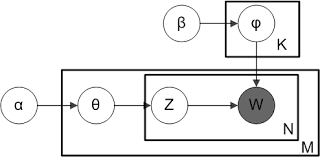
\includegraphics[scale=0.6]{Imgs/LDA.png}
\caption{مدل تخصیص پنهان دیریکله. روند تولید یک سند به طور کامل در این شکل مشخص است. هر سند شامل تعدادی کلمه است که در شکل با \lr{W} نشان داده‌ شده‌اند. کلمات با توجه به توزیع احتمالاتی شرطی کلمات به شرط عناوین (\lr{$\Theta$}) و بردار عناوین موجود در اسناد (\lr{Z}) به‌وجود می‌آید. بردار \lr{Z}، در شکل، با استفاده از توزیع احتمالاتی عناوین به شرط اسناد (\lr{$\Phi$}) تشکیل می‌شود. پارامترهای $\alpha$ و $\beta$، پارامترهای توزیع دیریکله برای تولید متغیرهای تصادفی $\alpha$ و $\beta$ هستند.}
\label{eq:lda}
\end{figure}

مراحل اجرای الگوریتم نمونه‌برداری گیبس در بخش یادگیری مدل به شرح زیر است:
($k$ تعداد عناوین موجود و $l$ تعداد کلمات موجود هستند.)

\begin{enumerate}
\item
 کلیه متغیرهای تصادفی $z_i$ با یک مقدار تصادفی بین ۱ تا $l$ مقداردهی می‌شوند. ($l$ تعداد کل کلمات موجود در مجموعه اسناد و $z_i$ عنوان پیشنهادی برای کلمه $w_i$ است.)
\item
تا زمانی که شرایط 
\lr{mixing}
 برقرار نشده مراحل زیر تکرار می‌شوند.
 \footnote{در این پروژه، شرایط \lr{mixing} پس از سپری شدن تعداد مشخصی تکرار ، احراز شده فرض می‌شود.}

\begin{enumerate}
\item 
به ازای تمام کلمات $w_i$، توزیع احتمالی تغییر عنوان به هریک از عناوین موجود، مطابق با رابطه \ref{eq:pzcond}
حساب می‌شود.
\begin{equation}
p(z_i = j | .) \propto \frac{n_{-i,j}^{w_i} + \beta }{n_{-i,j}^{.} + W \cdot \beta} \cdot \frac{n_{-i,j}^{d_i} + \alpha}{n_{-i,.}^{d_i} + l \cdot \alpha}
\label{eq:pzcond}
\end{equation}
\item
یک داده تصادفی از توزیع احتمالاتی $p(z_i = j | .)$  که در مرحله قبل محاسبه شده است، تولید شده و عنوان کلمه $w_i$ مساوی این مقدار جدید قرار می‌گیرد.
\item
ماتریس شمارش‌های محاسبه شده که در رابطه \ref{eq:pzcond} مورد استفاده قرار گرفته‌اند، تصحیح می‌شوند.
\end{enumerate}

\item
با توجه به قاعده نمونه‌برداری که در ادامه توضیح داده خواهد شد، یک نمونه از بردار $Z$ تولید می‌شود.
\item
با استفاده از نمونه تولید شده و با در نظر گرفتن روابط 
\ref{eq:theta}
و
\ref{eq:phi}
فاکتورهای $\Theta$ و $\Phi$ محاسبه می‌شوند.

\begin{equation}
\hat{\Theta}_{j}^{d} = \frac{n_j^d + \alpha}{n_{.}^d + k \cdot \alpha}
\label{eq:theta}
\end{equation}

\begin{equation}
\hat{\Phi}_{j}^{w} = \frac{n_j^w + \beta}{n_j^{.} + l \cdot \beta}
\label{eq:phi}
\end{equation}

\end{enumerate}


در ادامه به بررسی تاثیر پارامترهای مختلف بر عملکرد الگوریتم می‌پردازیم.

%%%%%%%%%%%%%%%%%%%%%%%%%%%%%%%%%%%%%%%%%%%%%%%%%%%%%%%%%%%%%%%%%%%%%%%%%%%%%%%%%%%
\subsection{پارامتر توزیع‌های دیریکله اولیه}

در این بخش قصد داریم تاثیر پارامترهای $\alpha$ و $\beta$ را بر عملکرد الگوریتم مورد بررسی قرار دهیم. در تمام آزمایشات این بخش، برای افزایش سرعت محاسبات، مقدار $k = 3$ در نظر گرفته شده است. همین‌طور ۷۰ درصد از کل داده‌ها به طور تصادفی به مجموعه آموزشی و ۳۰ درصد باقیمانده به مجموعه تست اختصاص داده‌ شده‌اند.

\subsubsection{تاثیر پارامتر آلفا}
مطابق با رابطه \ref{eq:theta}، که نحوه محاسبه فاکتور $\Theta$ را مشخص می‌کند، مقدار پارامتر $\alpha$ در توزیع احتمالی عناوین به شرط اسناد تاثیرگذار است. اگر این پارامتر را برابر با صفر در نظر بگیریم (رابطه \ref{eq:thetamle})، رابطه تبدیل به یک تخمین \lr{MLE} ساده (تعداد کلمات موجود از هر عنوان به کل عناوین موجود در بین کلمات یک سند) برای عناوین خواهد شد. با اضافه کردن پارامتر $\alpha$ به رابطه، به شکلی دانش اولیه خود را در تخمین توزیع‌ها دخالت داده‌ایم. رابطه \ref{eq:theta} دقیقا برابر با رابطه \ref{eq:thetamle} است در صورتی که خودمان به طور دستی به هر جمله $\alpha$ کلمه از همه عناوین وارد کرده باشیم. این کار معادل این است که در ابتدا احتمال رخداد تمام عناوین را در اسناد با یک‌دیگر برابر بدانیم. از طرفی هر چه مقدار $\alpha$ بزرگتر باشد، اطمینان ما از دانش اولیه بیشتر است و برعکس.

\begin{equation}
\hat{\Theta}_{j}^{d} = \frac{n_j^d }{n_{.}^d}
\label{eq:thetamle}
\end{equation}

با توجه به توضیحات ارائه شده، انتظار می‌رود، با کاهش میزان $\alpha$ مدل با سرعت بیشتری به داده‌ها برازش شود. اگر مقدار این پارامتر خیلی کوچک باشد، احتمال وقوع بیش‌برازش\enfootnote{Overfit} به داده‌ها به طور چشم‌گیری افزایش خواهد یافت. از طرفی اگر مقدار این پارامتر، به طور قابل توجهی بزرگ باشد، اطمینان بالای ما از دانش اولیه را نشان می‌دهد. این مساله باعث خواهد شد، قدرت یادگیری مدل از داده‌ها کاهش یافته و مدل نتواند توزیع‌های واقعی موجود در مجموعه اسناد موجود را به درستی نمایش دهد.
\\

آزمایشات انجام شده در این بخش، مؤید انتظارات ما از نحوه رفتار پارامتر است. جدول \ref{tbl:alpha}
نتایج عملکرد الگوریتم را به ازای مقادیر مختلف از پارامتر $\alpha$ نمایش می‌دهد. در تمام موارد $\beta = 0.5$ است.
\begin{table}[h]
\center
\caption{تاثیر پارامتر $\alpha$ در عملکرد الگوریتم}
\label{tbl:alpha}
\begin{tabular}{c | c | c | c}
$\alpha$ & زمان سپری شده در هر تکرار & سرگشتگی\enfootnote{Perplexity} مجموعه آموزشی & سرگشتگی مجموعه تست\\
\hline
\hline
0.01 & 25 & 3615.648 & 4212.840 \\
0.03 & 25 & 3648.938 & 4205.395 \\
0.1 & 25 & 3683.480 & 4170.122 \\
\end{tabular}
\end{table}

همان‌طور که نتایج جدول \ref{tbl:alpha} نمایش می‌دهند با کاهش مقدار این پارامتر، میزان سرگشتگی الگوریتم روی مجموعه آموزشی کاهش می‌یابد. بر خلاف نتایج مجموعه آموزشی، سرگشتگی الگوریتم در بین داده‌های تست تا نقطه‌ای کاهش یافته و با کاهش بیش از حد مقدار این پارامتر، دوباره افزایش می‌یابد. این نکته نشان می‌دهد کاهش بیش از حد مقدار این پارامتر، باعث ایجاد بیش‌برازش بر داده‌ها می‌شود. بهترین مقدار به‌دست آمده برای این پارامتر،‌ $\alpha = 0.3$
است.

شکل 
\ref{fig:alpha}
نمودار تغییرات سرگشتگی مدل را به ازای مقادیر مختلف پارامتر $\alpha$ روی مجموعه‌های آموزشی و تست نمایش می‌دهد.

\begin{figure}[h]
\center
	\begin{subfigure}{.45\textwidth}
%		\center
		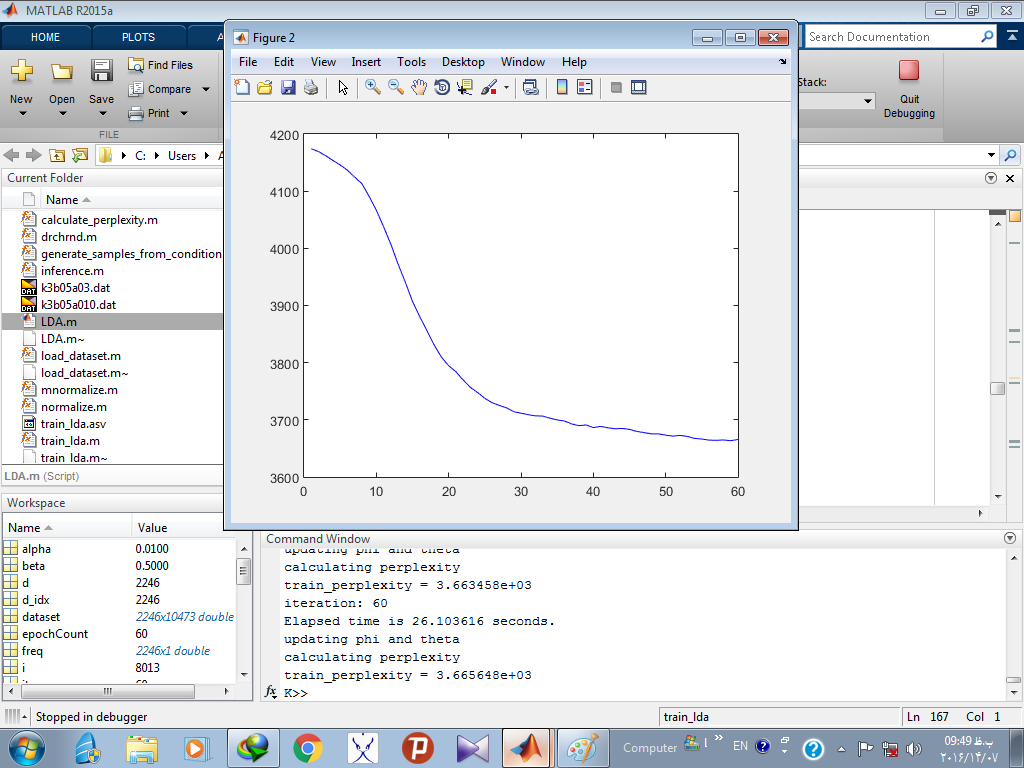
\includegraphics[scale=0.25]{Imgs/k3_b05_a001_25s_ptr3665648.png}
		\caption{نمودار تغییرات سرگشتگی مجموعه‌ آموزشی با $\alpha = 0.01$}
	\end{subfigure}
	\begin{subfigure}{.45\textwidth}
%		\center
		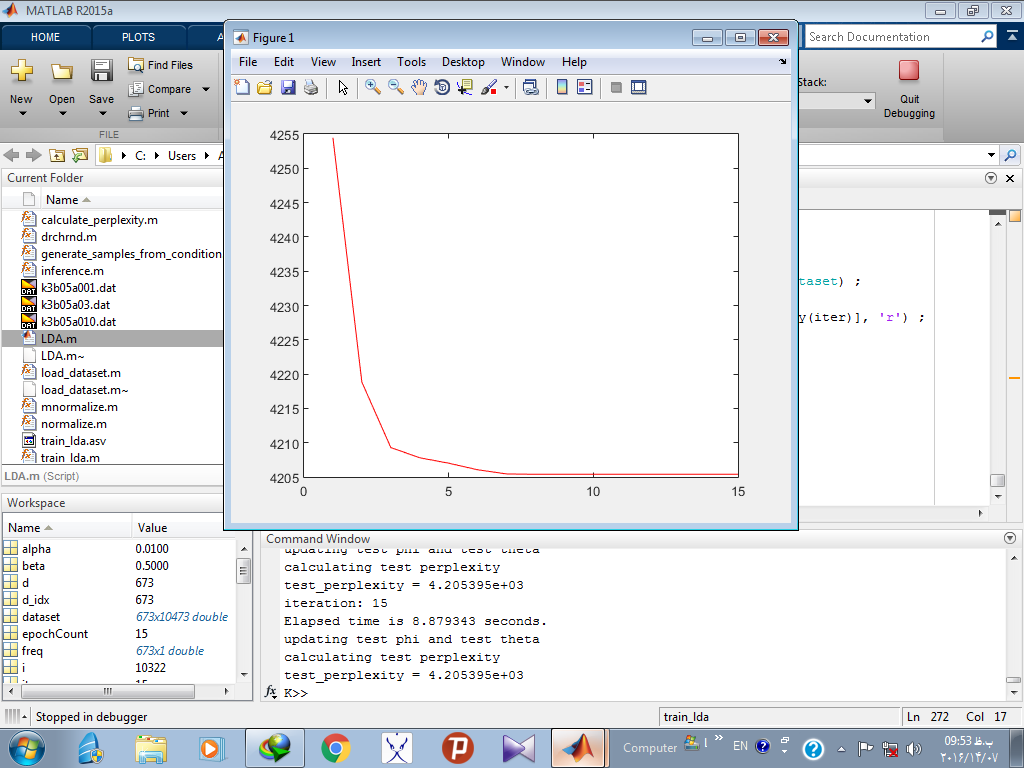
\includegraphics[scale=0.25]{Imgs/k3_b05_a001_8s_pts4205395.png}
		\caption{نمودار تغییرات سرگشتگی مجموعه‌ تست با $\alpha = 0.01$}
	\end{subfigure}

	\begin{subfigure}{.45\textwidth}
%		\center
		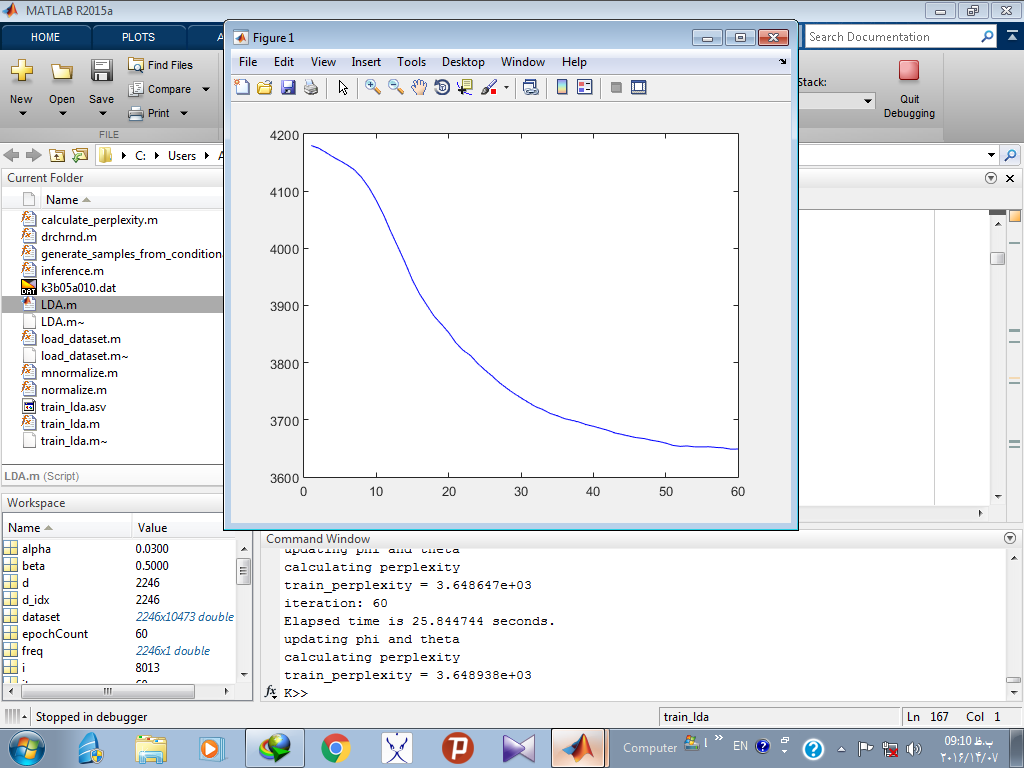
\includegraphics[scale=0.25]{Imgs/k3_b05_a003_25s_ptr3648938.png}
		\caption{نمودار تغییرات سرگشتگی مجموعه‌ آموزشی با $\alpha = 0.03$}
	\end{subfigure}
	\begin{subfigure}{.45\textwidth}
%		\center
		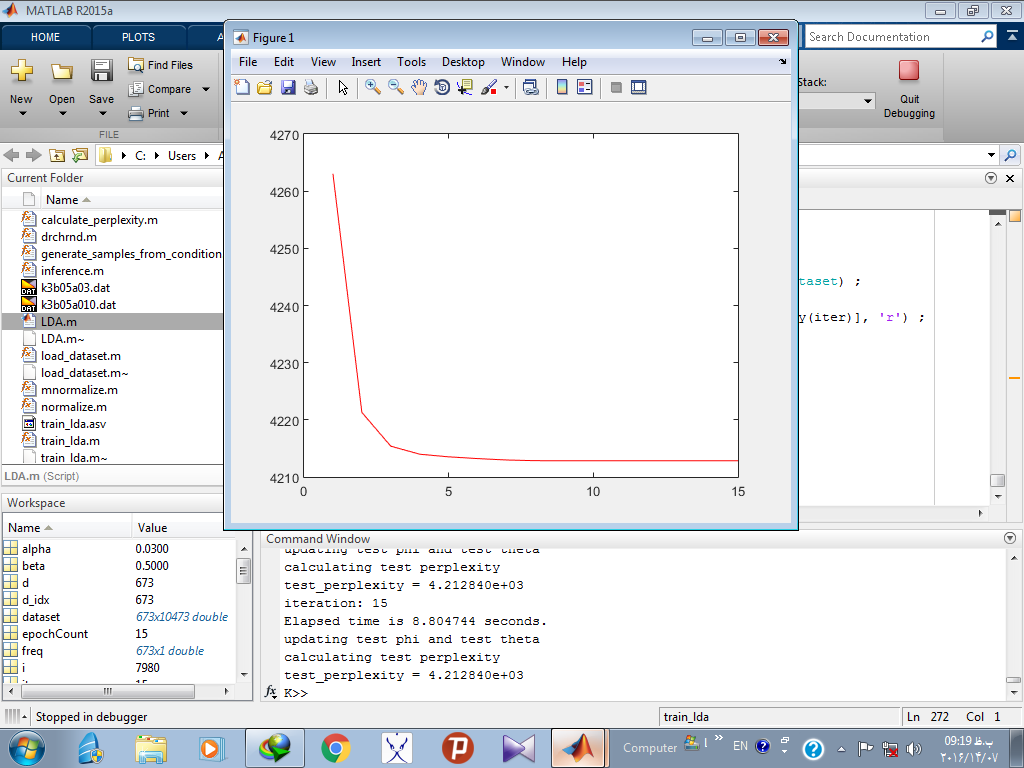
\includegraphics[scale=0.25]{Imgs/k3_b05_a003_8s_pts4212840.png}
		\caption{نمودار تغییرات سرگشتگی مجموعه‌ تست با $\alpha = 0.03$}
	\end{subfigure}

	\begin{subfigure}{.45\textwidth}
%		\center
		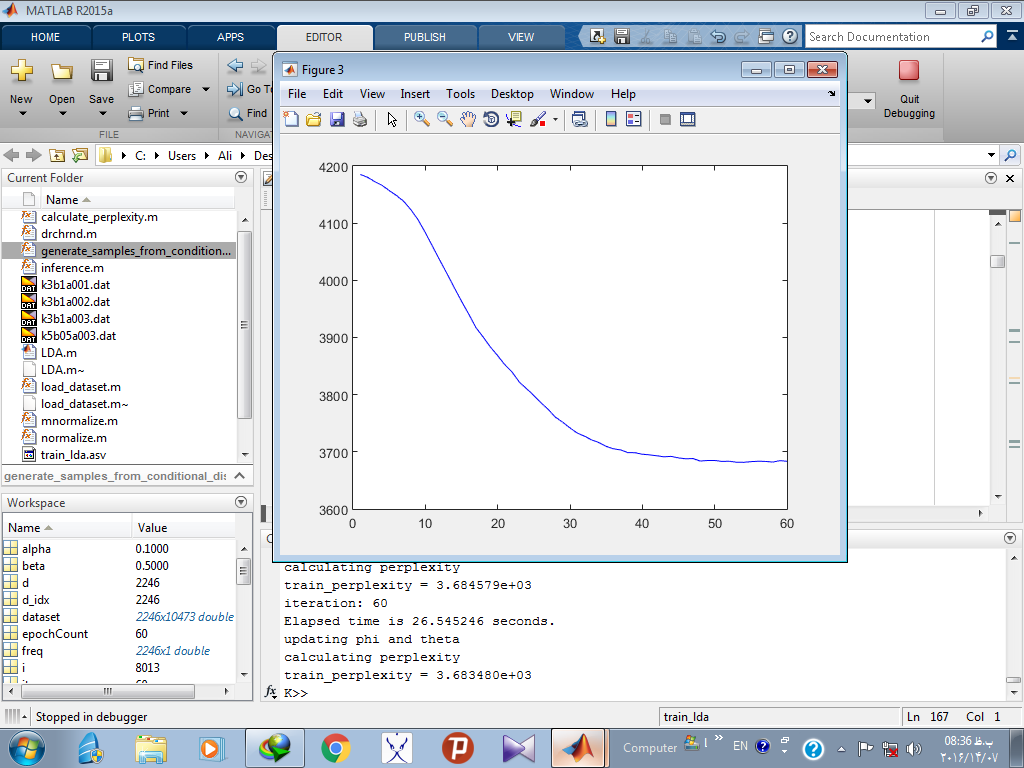
\includegraphics[scale=0.25]{Imgs/k3_b05_a010_26s_ptr3683480.png}
		\caption{نمودار تغییرات سرگشتگی مجموعه‌ آموزشی با $\alpha = 0.1$}
	\end{subfigure}
	\begin{subfigure}{.45\textwidth}
%		\center
		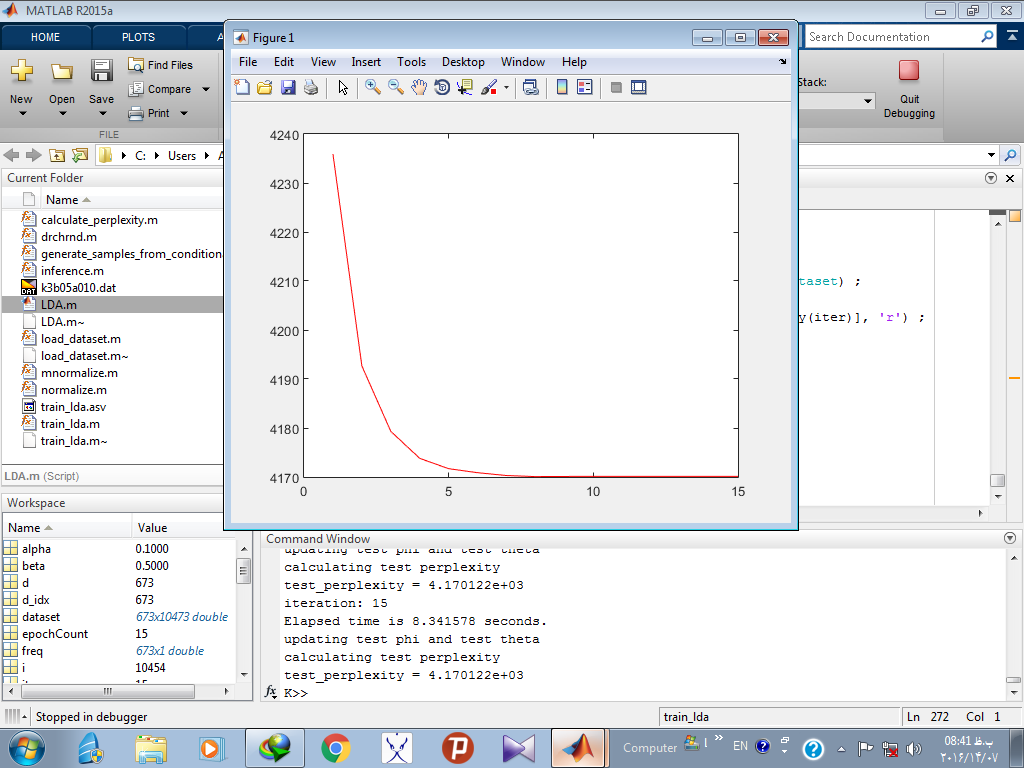
\includegraphics[scale=0.25]{Imgs/k3_b05_a010_8s_pts4170122.png}
		\caption{نمودار تغییرات سرگشتگی مجموعه‌ تست با $\alpha = 0.1$}
	\end{subfigure}
\caption{تغییرات سرگشتگی مدل به ازای مقادیر مختلف پارامتر $\alpha$ برای مجموعه‌های آموزشی و تست
}
\label{fig:alpha}
\end{figure} 

\subsubsection{تاثیر پارامتر بتا}
مانند پارامتر آلفا می‌توان در مورد پارامتر بتا نیز قضاوت کرد. مطابق با رابطه \ref{eq:phi}، که نحوه محاسبه فاکتور $\Phi$ را مشخص می‌کند، مقدار پارامتر $\beta$ در توزیع احتمالی کلمات به شرط عناوین تاثیرگذار است. اگر این پارامتر را برابر با صفر در نظر بگیریم (رابطه \ref{eq:phimle})، رابطه تبدیل به یک تخمین \lr{MLE} ساده (تعداد کلمات موجود از هر عنوان در بین کل کلمات موجود در مجموعه اسناد) برای کلمات خواهد شد. با اضافه کردن پارامتر $\beta$ به رابطه، به شکلی دانش اولیه خود را در تخمین توزیع‌ها دخالت داده‌ایم. رابطه \ref{eq:phi} دقیقا برابر با رابطه \ref{eq:phimle} است در صورتی که خودمان به طور دستی  $\beta$ کلمه از همه عناوین وارد مجموعه اسناد موجود، کرده باشیم. این کار معادل این است که در ابتدا احتمال رخداد تمام کلمات را در عناوین با یک‌دیگر برابر بدانیم. از طرفی هر چه مقدار $\beta$ بزرگتر باشد، اطمینان ما از دانش اولیه بیشتر است و برعکس.

\begin{equation}
\hat{\Phi}_{j}^{d} = \frac{n_j^w }{n_{j}^{(.)}}
\label{eq:phimle}
\end{equation}

جدول \ref{tbl:beta}
نتایج عملکرد الگوریتم را به ازای مقادیر مختلف از پارامتر $\beta$ نمایش می‌دهد. 
\begin{table}[h]
\center
\caption{تاثیر پارامتر $\beta$ در عملکرد الگوریتم}
\label{tbl:beta}
\begin{tabular}{c | c | c | c}
$\beta$ & زمان سپری شده در هر تکرار & سرگشتگی\enfootnote{Perplexity} مجموعه آموزشی & سرگشتگی مجموعه تست\\
\hline
\hline
0.5 & 25 & 3648.938 & 4205.395 \\
1 & 25 & 3672.436 & 4133.398 \\
2 & 25 & 3758.397 & 4217.278 \\
\end{tabular}
\end{table}

همان‌طور که نتایج جدول \ref{tbl:beta} نمایش می‌دهند پارامتر $\beta$ نیز مانند پارامتر $\alpha$ عمل می‌کند. بهترین مقدار به‌دست آمده برای این پارامتر، $\beta = 1$ است.
شکل 
\ref{fig:beta}
نمودار تغییرات سرگشتگی مدل را به ازای مقادیر مختلف پارامتر $\beta$ روی مجموعه‌های آموزشی و تست نمایش می‌دهد.

\begin{figure}[h]
\center
	\begin{subfigure}{.45\textwidth}
%		\center
		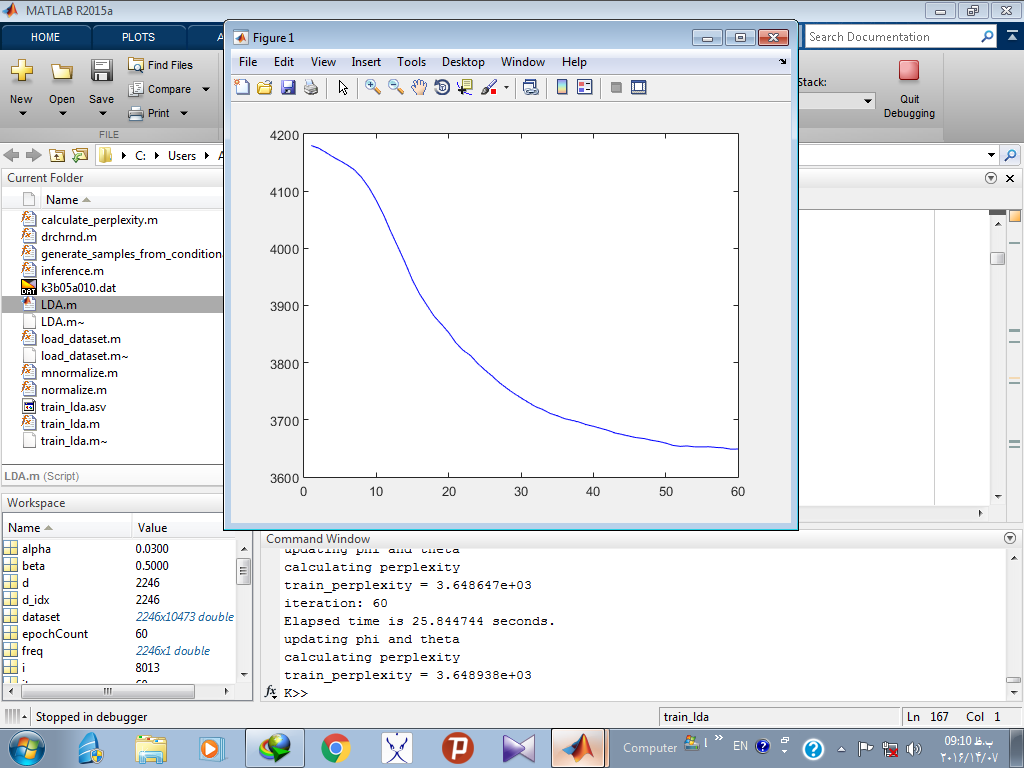
\includegraphics[scale=0.25]{Imgs/k3_b05_a003_25s_ptr3648938.png}
		\caption{نمودار تغییرات سرگشتگی مجموعه‌ آموزشی با $\beta = 0.5$}
	\end{subfigure}
	\begin{subfigure}{.45\textwidth}
%		\center
		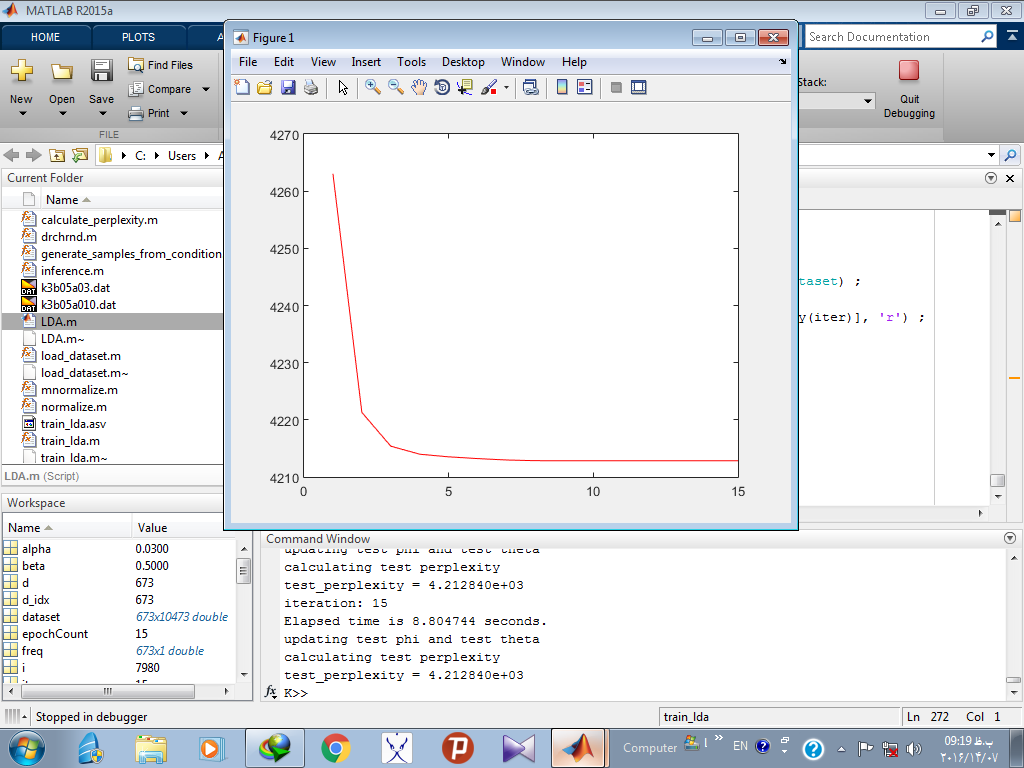
\includegraphics[scale=0.25]{Imgs/k3_b05_a003_8s_pts4212840.png}
		\caption{نمودار تغییرات سرگشتگی مجموعه‌ تست با $\beta = 0.5$}
	\end{subfigure}

	\begin{subfigure}{.45\textwidth}
%		\center
		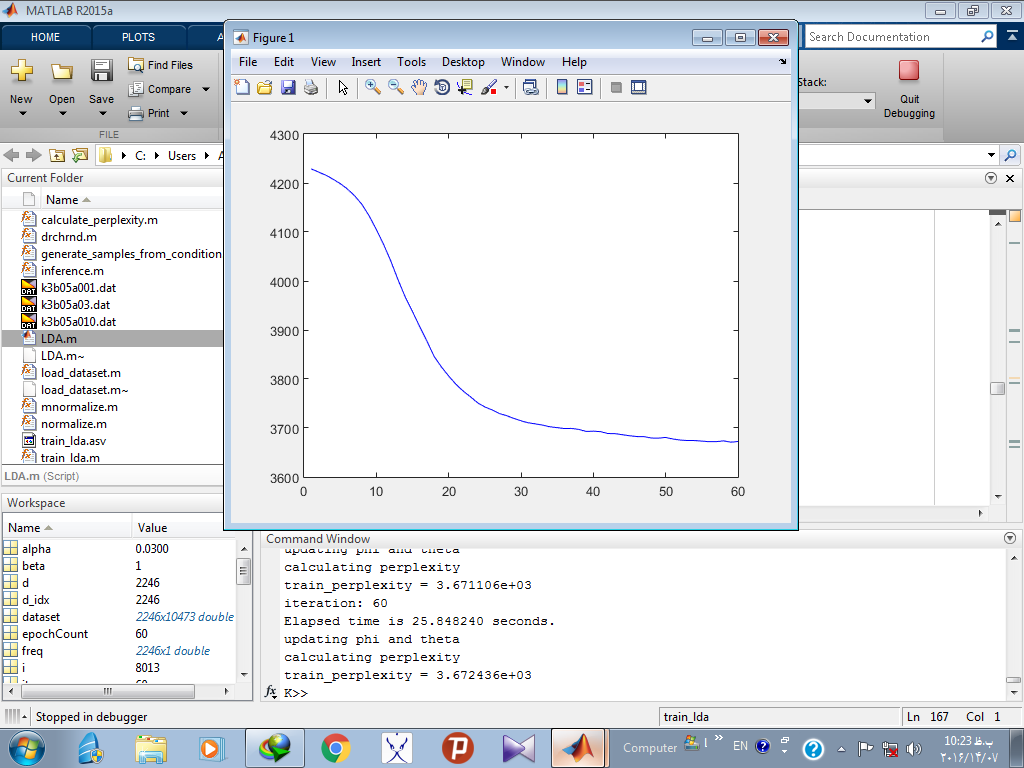
\includegraphics[scale=0.25]{Imgs/k3_b1_a003_25s_ptr3672436.png}
		\caption{نمودار تغییرات سرگشتگی مجموعه‌ آموزشی با $\beta = 1$}
	\end{subfigure}
	\begin{subfigure}{.45\textwidth}
%		\center
		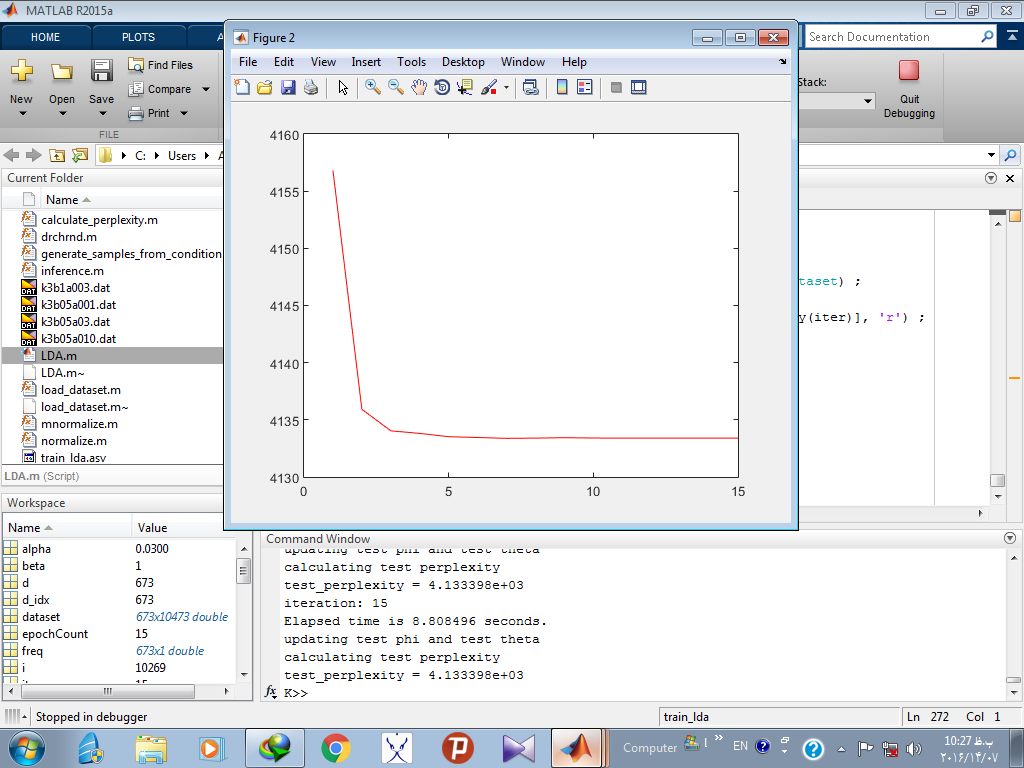
\includegraphics[scale=0.25]{Imgs/k3_b1_a003_8s_pts4133398.png}
		\caption{نمودار تغییرات سرگشتگی مجموعه‌ تست با $\beta = 1$}
	\end{subfigure}

	\begin{subfigure}{.45\textwidth}
%		\center
		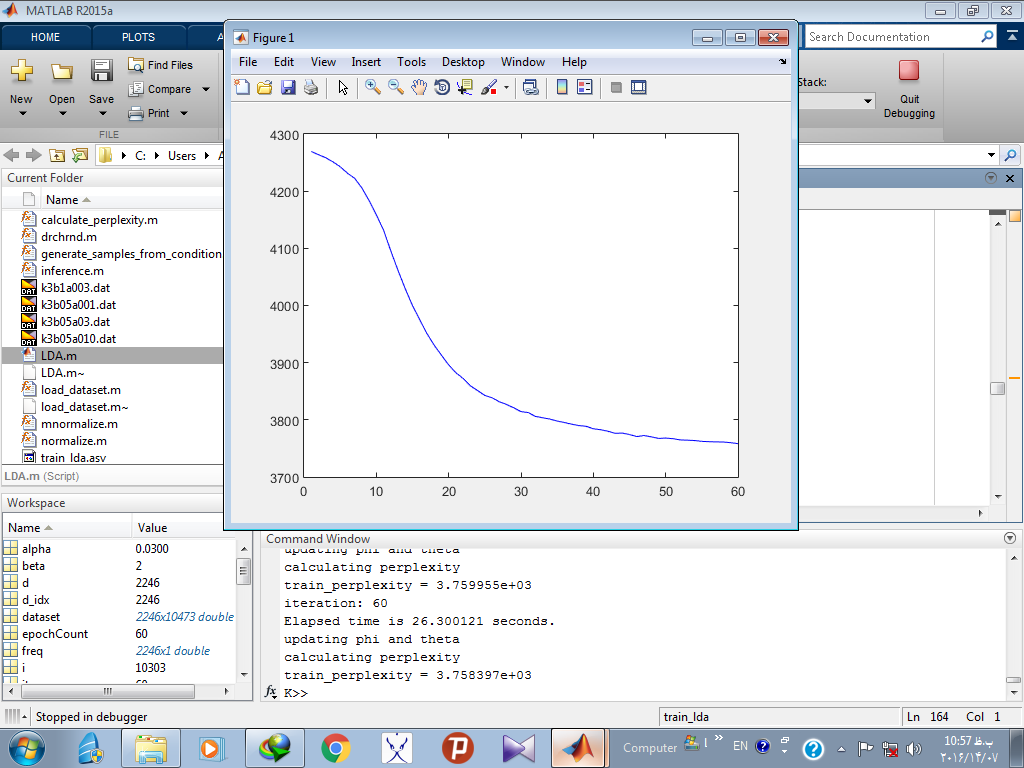
\includegraphics[scale=0.25]{Imgs/k3_b2_a003_25s_ptr3758397.png}
		\caption{نمودار تغییرات سرگشتگی مجموعه‌ آموزشی با $\beta = 2$}
	\end{subfigure}
	\begin{subfigure}{.45\textwidth}
%		\center
		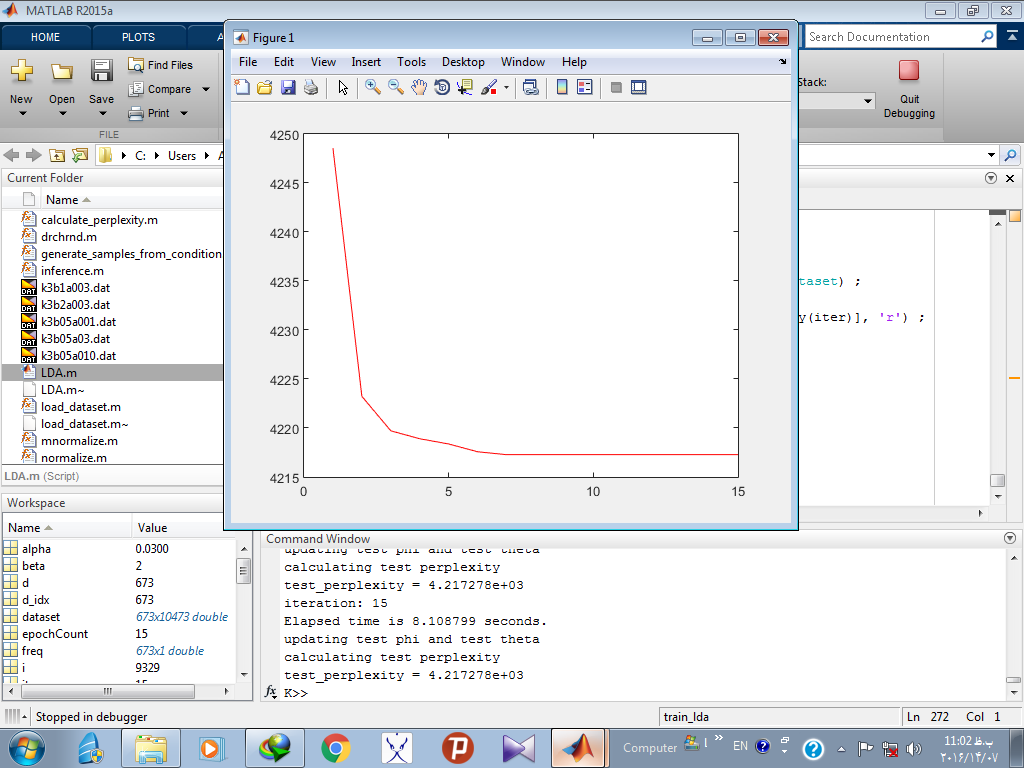
\includegraphics[scale=0.25]{Imgs/k3_b2_a003_8s_pts4217278.png}
		\caption{نمودار تغییرات سرگشتگی مجموعه‌ تست با $\beta = 2$}
	\end{subfigure}
\caption{تغییرات سرگشتگی مدل به ازای مقادیر مختلف پارامتر $\beta$ برای مجموعه‌های آموزشی و تست
}
\label{fig:beta}
\end{figure} 




%%%%%%%%%%%%%%%%%%%%%%%%%%%%%%%%%%%%%%%%%%%%%%%%%%%%%%%%%%%%%%%%%%%%%%%%%%%%%%%%%%%
\subsection{تاثیر تعداد عناوین}

مطابق با آزمایشات انجام شده، با افزایش تعداد عناوین، عملکرد الگوریتم بهبود یافت. البته انتظار می‌رود با افزایش بیش از حد تعداد عناوین، مانند حالتی که در خوشه‌بندی داده‌ها تعداد خوشه‌های از پیش تعیین شده بسیار زیاد است، الگوریتم دچار بیش‌برازش شود که به دلیل زمان‌بر بودن این حالت (هر تکرار حدود 980 ثانیه با تعداد 100 عنوان) امکان تست آن فراهم نشد.
\\
مطابق با نمودارهای به‌دست آمده از این بخش، هرچه تعداد عناوین افزایش می‌یابد، سرگشتگی اولیه الگوریتم نیز بالاتر می‌رود. این امر، کاملا قابل انتظار است زیرا از آنجا که تعداد عناوین زیاد است، با شروع از یک نقطه تصادفی و یک مرحله تکرار، احتمال اشتباه بودن عنوان تخصیص یافته شده به اسناد و کلمات بیشتر است تا زمانی که تعداد عناوین کم باشد.
\\
 از طرف دیگر سرعت همگرا شدن الگوریتم با بالا رفتن تعداد عناوین، افزایش می‌یابد. این مورد هم با در نظر گرفتن این که با افزایش تعداد عناوین، نیاز به تعمیم درون‌گروهی هر عنوان کاهش می‌یابد، به راحتی قابل توجیه است. هر چه تعداد عناوین افزایش یابد، اسناد کمتری در یک خوشه قرار می‌گیرند. از آنجا که یافتن تعداد کم، سندی که شباهت زیادی به یکدیگر دارند، راحت‌تر از یافتن تعداد زیاد سند شبیه به هم است، شباهت اسناد درون یک عنوان در حالتی که تعداد عناوین زیاد است، به مراتب بیشتر از حالات دیگر خواهد بود. با طی تعداد کمی تکرار، بسیاری از اسناد شبیه به هم موجود، تحت عناوین مشترک بیان می‌شوند و باعث بالا رفتن سرعت الگوریتم می‌شود.


جدول \ref{tbl:topics} نتایج تاثیر تعداد عناوین بر عملکرد الگوریتم را نمایش می‌دهد.

\begin{table}[h]
\center
\caption{تاثیر تعداد عناوین در عملکرد الگوریتم}
\label{tbl:topics}
\begin{tabular}{c | c | c | c}
تعداد عناوین & زمان سپری شده در هر تکرار & سرگشتگی\enfootnote{Perplexity} مجموعه آموزشی & سرگشتگی مجموعه تست\\
\hline
\hline
3 & 25 & 3648.938 & 4205.395 \\
5 & 42 & 3524.945 & 4155.610 \\
10 & 135 & 3218.842 & 4407.000 \\
100 & 980 & محاسبه نشد & محاسبه نشد \\
\end{tabular}
\end{table}

شکل 
\ref{fig:topics}
نمودار تغییرات سرگشتگی الگوریتم بر اساس تعداد عناوین را نمایش می‌دهد.


\begin{figure}[h]
\center
	\begin{subfigure}{.45\textwidth}
%		\center
		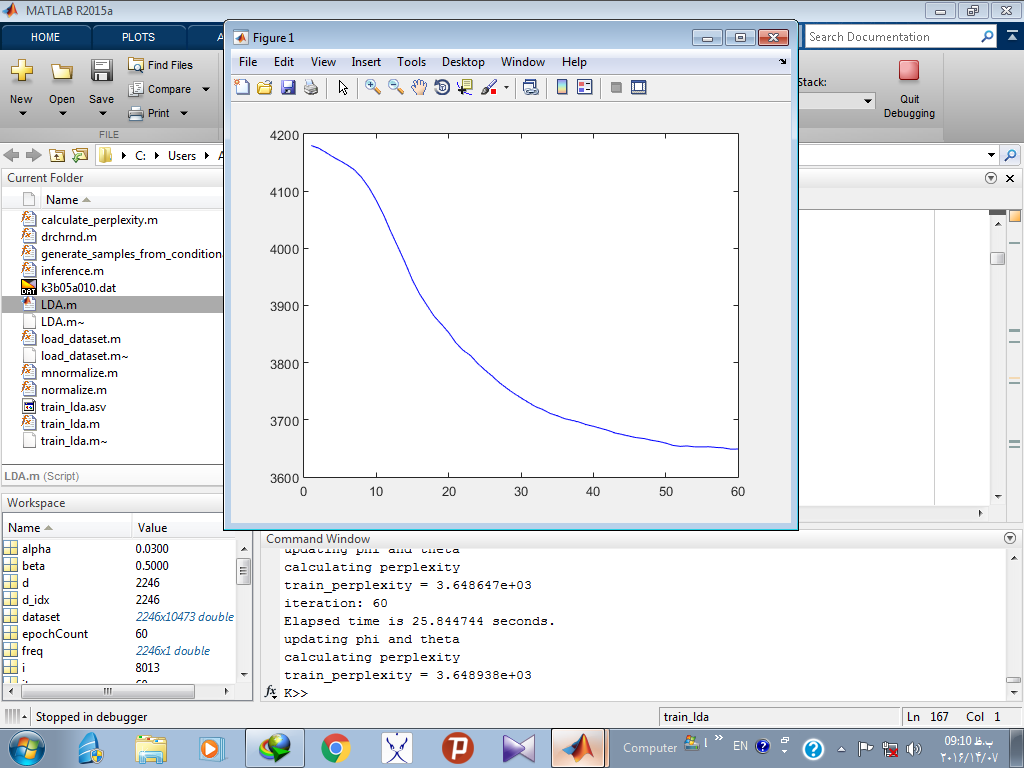
\includegraphics[scale=0.25]{Imgs/k3_b05_a003_25s_ptr3648938.png}
		\caption{نمودار تغییرات سرگشتگی مجموعه‌ آموزشی با ۳ عنوان}
	\end{subfigure}
	\begin{subfigure}{.45\textwidth}
%		\center
		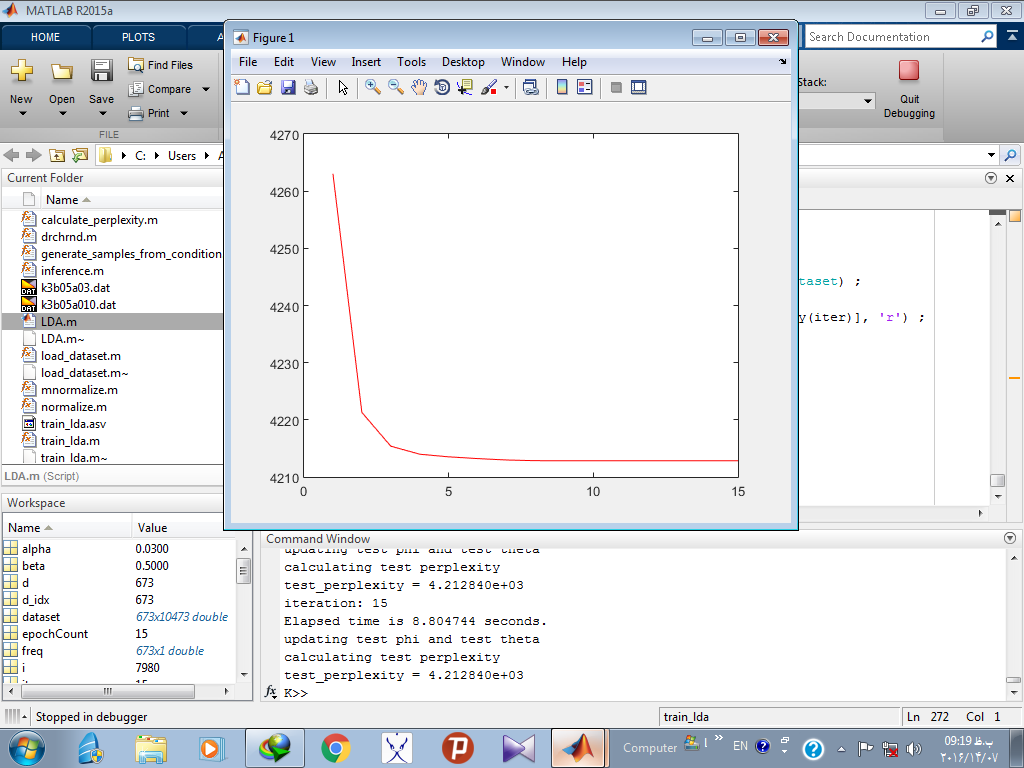
\includegraphics[scale=0.25]{Imgs/k3_b05_a003_8s_pts4212840.png}
		\caption{نمودار تغییرات سرگشتگی مجموعه‌ تست با ۳ عنوان}
	\end{subfigure}

	\begin{subfigure}{.45\textwidth}
%		\center
		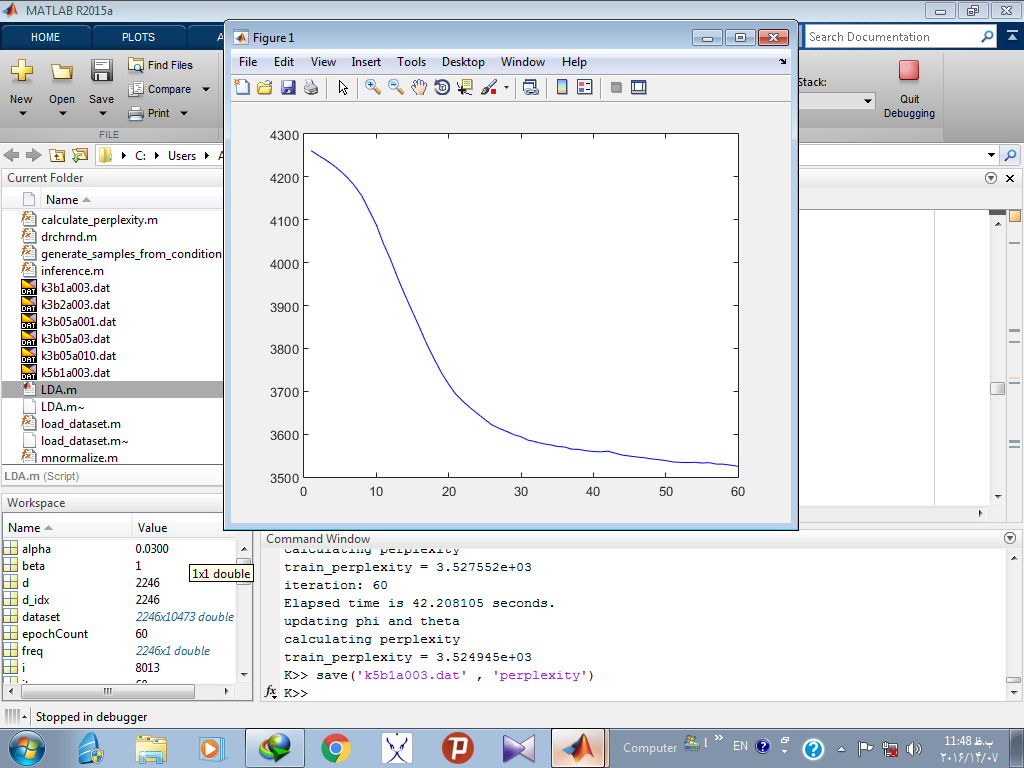
\includegraphics[scale=0.25]{Imgs/k5_b1_a003_25s_ptr3524945.png}
		\caption{نمودار تغییرات سرگشتگی مجموعه‌ آموزشی با ۵ عنوان}
	\end{subfigure}
	\begin{subfigure}{.45\textwidth}
%		\center
		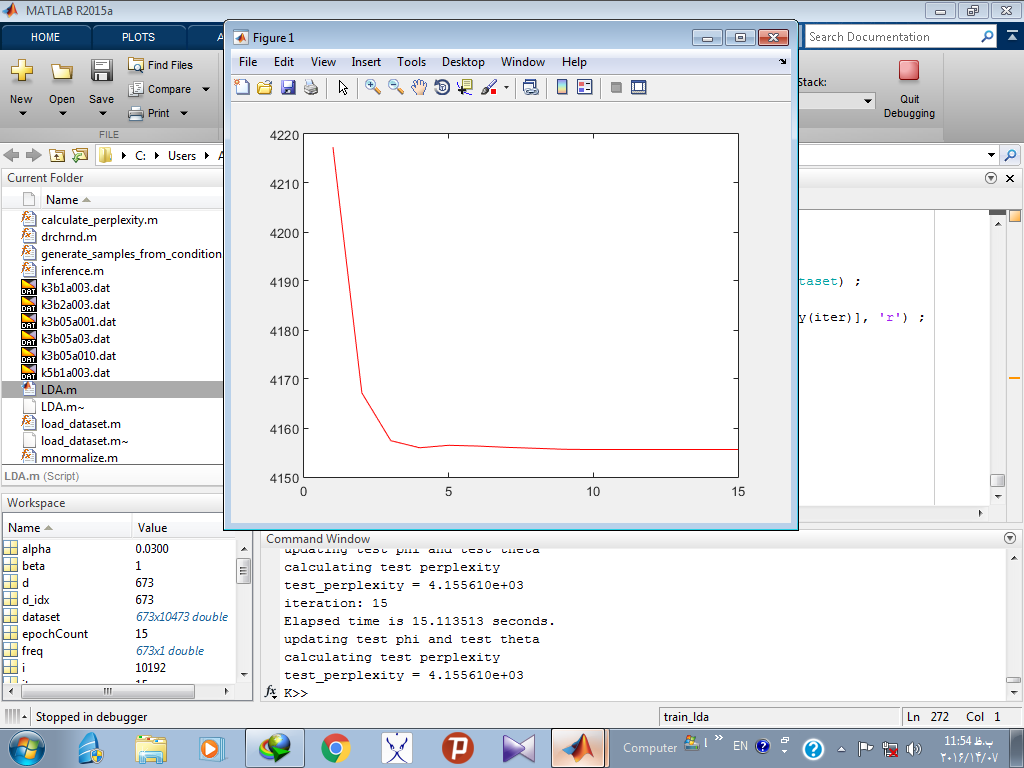
\includegraphics[scale=0.25]{Imgs/k5_b1_a003_8s_pts4155610.png}
		\caption{نمودار تغییرات سرگشتگی مجموعه‌ تست با ۵ عنوان}
	\end{subfigure}

	\begin{subfigure}{.45\textwidth}
%		\center
		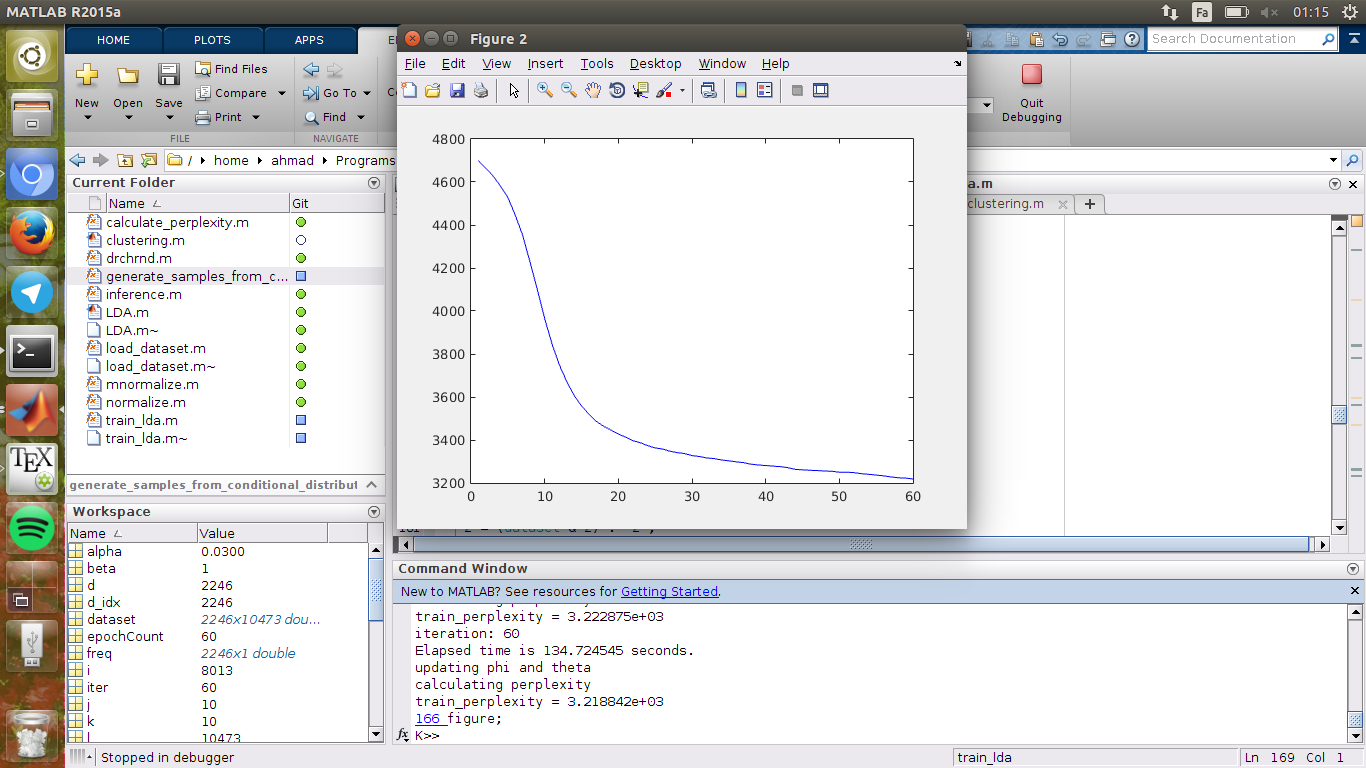
\includegraphics[scale=0.2]{Imgs/k10_b1_a004_134s_ptr3218842.png}
		\caption{نمودار تغییرات سرگشتگی مجموعه‌ آموزشی با 10 عنوان}
	\end{subfigure}
	\begin{subfigure}{.45\textwidth}
%		\center
		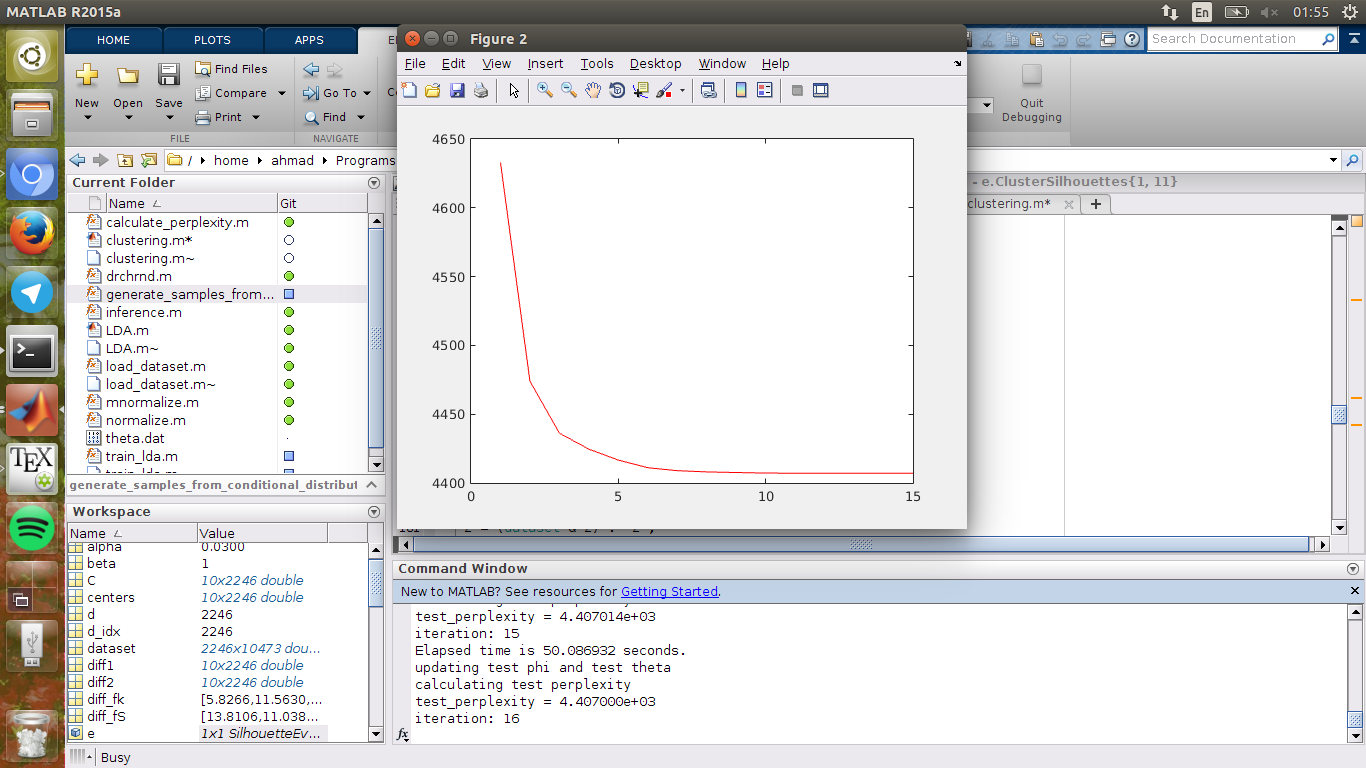
\includegraphics[scale=0.2]{Imgs/k10_b1_a003_51s_pts4407000.png}
		\caption{نمودار تغییرات سرگشتگی مجموعه‌ تست با 10 عنوان}
	\end{subfigure}
\caption{تغییرات سرگشتگی مدل به ازای تعداد عناوین مختلف برای مجموعه‌های آموزشی و تست
}
\label{fig:topics}
\end{figure} 




%%%%%%%%%%%%%%%%%%%%%%%%%%%%%%%%%%%%%%%%%%%%%%%%%%%%%%%%%%%%%%%%%%%%%%%%%%%%%%%%%%%
\subsection{تاثیر روند نمونه‌برداری}
پس از رسیدن به شرایط \lr{mixing}، بردار $Z$ مورد استفاده برای محاسبه فاکتورهای مدل، از طریق فرایند نمونه‌برداری تولید می‌شود. روش‌های مختلف موجود برای این کار، به شرح زیر می‌باشند.

\begin{enumerate}
\item 
استفاده از آخرین نمونه تولید شده $Z$
\item 
استفاده از چند نمونه آخر تولید شده $Z$
\item
استفاده از تعدادی از چند نمونه آخر تولید شده $Z$
\end{enumerate}

روش اول، ساده‌ترین روش ممکن برای این کار است. در این روش پس از رسیدن به \lr{mixing}، از نمونه $Z$ تولید شده به طور مستقیم برای محاسبات بعدی استفاده می‌شود. در این روش، پس از اتمام تمام تکرارها و تولید یک نمونه $Z$، 
دوباره باید از ابتدا الگوریتم را شروع کرده و انجام دهیم تا به \lr{mixing} برسیم و سپس یک نمونه $Z$ دیگر تولید کنیم تا به تعداد دلخواه نمونه $Z$ برسیم. همان‌طور که مشخص است این روش در این پروژه قابل انجام نیست. (به دلیل صرف زمان بسیار زیاد)
\\
 در روش دوم پس از رسیدن به \lr{mixing}، به تعداد دلخواه تکرار ها را ادامه می‌دهیم تا نمونه‌های $Z$ دلخواه تولید شوند و سپس با در دست داشتن این نمونه‌ها، می‌توانیم محاسبات فاکتورها را انجام دهیم.
ایراد این روش، این است که نمونه‌های تولید شده در آن می‌توانند از هم مستقل نباشند. در این صورت، نمونه‌های تولید شده به یکدیگر وابسته هستند و یادگیری به درستی اتفاق نمی‌افتد. انتظار داریم در صورتی که نمونه‌های تولید شده در واقع از هم مستقل نباشند، عملکرد الگوریتم روی داده‌های تست بسیار ضعیف‌تر از عملکرد الگوریتم روی داده‌های آموزشی باشد.
\\
در روش سوم پس از ادامه دادن تکرار‌های الگوریتم به تعداد دلخواه پس از \lr{mixing}، تعدادی از نمونه‌ها را به طور تصادفی یا با فواصل یکسان انتخاب کرده و از آن‌ها برای محاسبات بعدی استفاده می‌کنیم. این روش مشکل روش‌های قبلی را برطرف می‌سازد.
\\
جدول 
\ref{tbl:clusters}
تاثیر نحوه نمونه‌برداری را بر عملکرد الگوریتم مشخص می‌کند. همان‌طور که پیداست اگر چه تفاوت‌های جزئی در بین روش‌ها مشخص است اما به نظر می‌رسد از آنجا که تعداد نمونه‌های انتخاب شده (2000 نمونه) بالا بوده و همین‌طور وابستگی موجود بین نمونه‌های پشت سرهم در روند مساله بی‌تاثیر یا کم‌تاثیر به نظر می‌رسد، بهبود قابل توجهی از نتایج قابل استنتاج نیست.

\begin{table}[h]
\center
\caption{تاثیر نحوه نمونه‌برداری در عملکرد الگوریتم}
\label{tbl:clusters}
\begin{tabular}{c | c | c }
نحوه نمونه‌برداری & سرگشتگی\enfootnote{Perplexity} مجموعه آموزشی & سرگشتگی مجموعه تست\\
\hline
\hline
روش دوم & 3648.938 & 4205.395 \\
روش سوم  با فواصل ۲ تایی & 3524.324 & 4328.595 \\
روش سوم  با فواصل ۴ تایی & 3573.924 & 4293.856 \\
\end{tabular}
\end{table}

\subsection{خوشه‌بندی}
در این بخش، فاکتور $\Theta$ برای خوشه‌بندی اسناد مورد استفاده قرار گرفته است. خوشه‌بندی اسناد با استفاده از روش \lr{KMeans} انجام و با استفاده از معیارهای \lr{CalinskiHarabasz} و \lr{silhouette} برای 20 خوشه، ارزیابی شده است. نتایج بدست آمده از این ارزیابی نشان می‌دهد استفاده از فاکتور $\Theta$ برای خوشه‌بندی داده‌ها (آموزش با ۱۰ عنوان) در ۱۶ خوشه، نتیجه بهینه را می‌دهد.
\\
همین‌طور شکل
\ref{fig:wordcluster}
و 
جدول
\ref{tbl:wordcluster}
در حالتی که از ۵ عنوان برای مدل استفاده شده است، ۱۰ مورد از کلمات شاخص هر عنوان را نمایش می‌دهند. همان‌طور که در شکل مشخص است، کلمات به خوبی از یک‌دیگر جدا شده‌اند و عنوان هر یک از ۵ گروه کلمه به طور واضح قابل تشخیص و تمیز از دیگر عناوین است که نشان‌دهنده عملکرد مناسب الگوریتم می‌باشد.

\begin{table}[h]
\center
\caption{کلمات نمونه از ۵ عنوان مشخص شده}
\label{tbl:wordcluster}
\begin{tabular}{c | c | c | c | c}
عنوان اول & عنوان دوم & عنوان سوم & عنوان چهارم & عنوان پنجم
\\
\hline
\hline
\lr{foreign} & \lr{things} & \lr{miles} & \lr{judge} & \lr{prices} \\
\lr{campaign} & \lr{really} & \lr{area} & \lr{convicted} & \lr{higher} \\
\lr{administration} & \lr{cant} & \lr{southern} & \lr{jury} & \lr{rose} \\
\lr{meeting} & \lr{doesnt} & \lr{shot} & \lr{guilty} & \lr{trading} \\
\lr{support} & \lr{mother} & \lr{soldiers} & \lr{alleged} & \lr{exchange} \\
\lr{minister} & \lr{feel} & \lr{fighting} & \lr{sentenced} & \lr{fell} \\
\lr{saying} & \lr{sure} & \lr{injured} & \lr{prosecutors} & \lr{average} \\
\lr{leader} & \lr{friends} & \lr{navy} & \lr{appeals} & \lr{points} \\
\lr{leaders} & \lr{franks} & \lr{israeli} & \lr{enforcement} & \lr{index} \\
\lr{decision} & \lr{magazine} & \lr{hundreds} & \lr{bentsen} & \lr{analysts} \\
\end{tabular}
\end{table}



\begin{figure}[h]
\center
	\begin{subfigure}{.45\textwidth}
%		\center
		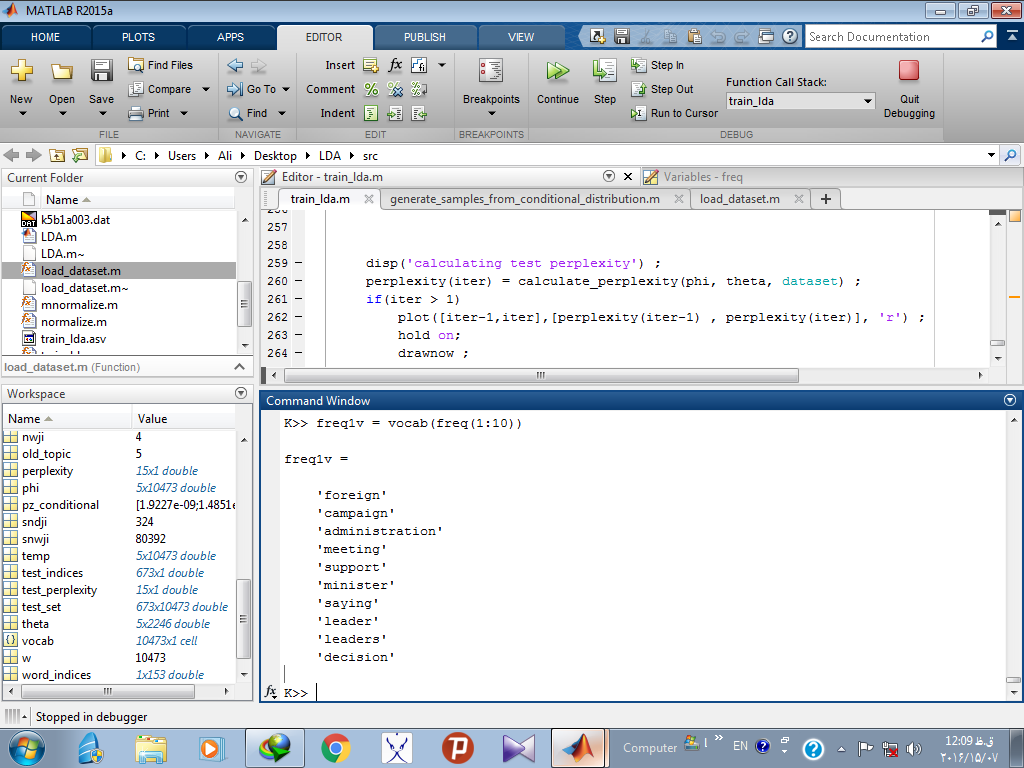
\includegraphics[scale=0.25]{Imgs/freqk1.png}
		\caption{کلمات شاخص عنوان اول}
	\end{subfigure}
	\begin{subfigure}{.45\textwidth}
%		\center
		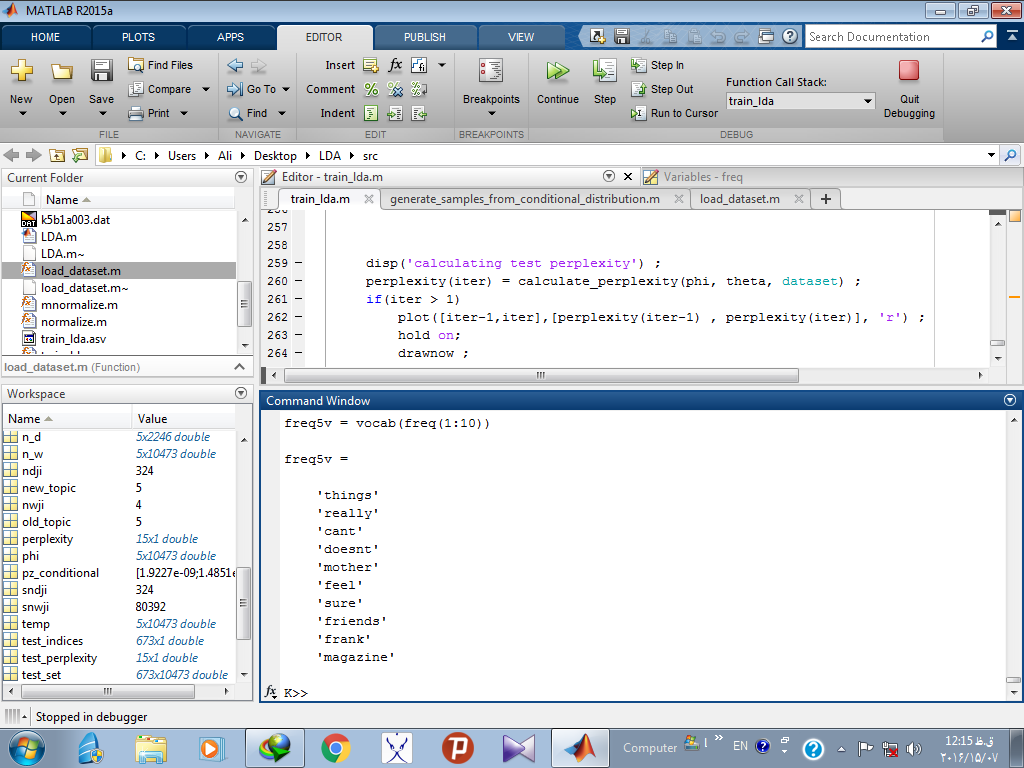
\includegraphics[scale=0.25]{Imgs/freqk2.png}
		\caption{کلمات شاخص عنوان دوم}
	\end{subfigure}

	\begin{subfigure}{.45\textwidth}
%		\center
		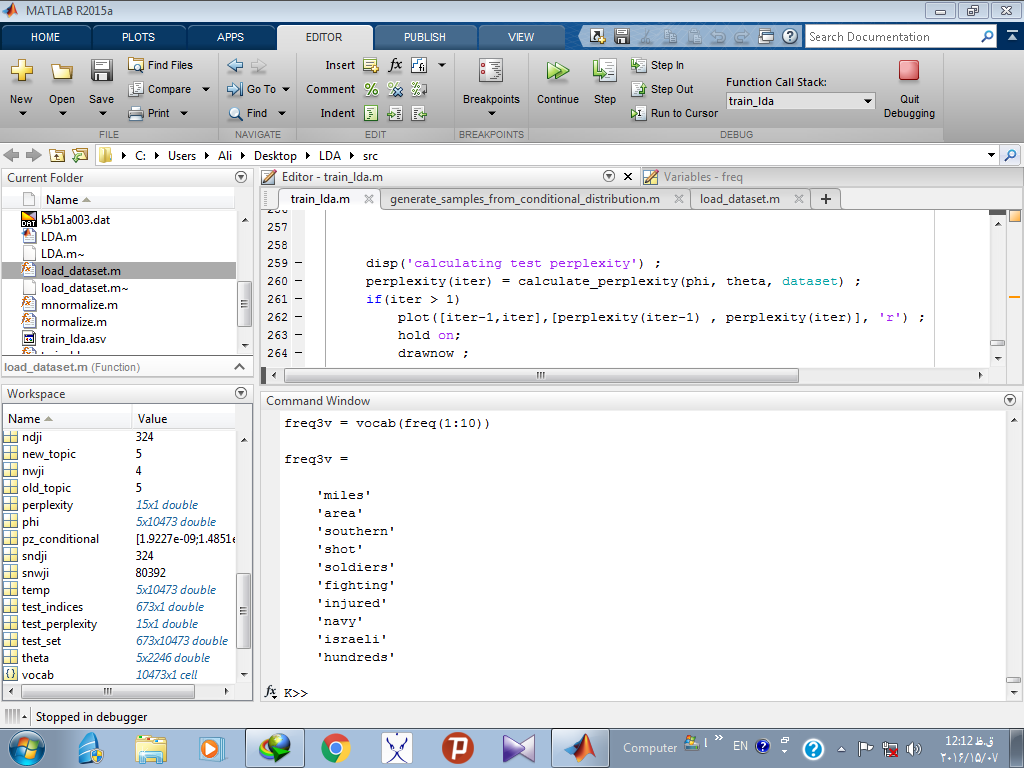
\includegraphics[scale=0.25]{Imgs/freqk3.png}
		\caption{کلمات شاخص عنوان سوم}
	\end{subfigure}
	\begin{subfigure}{.45\textwidth}
%		\center
		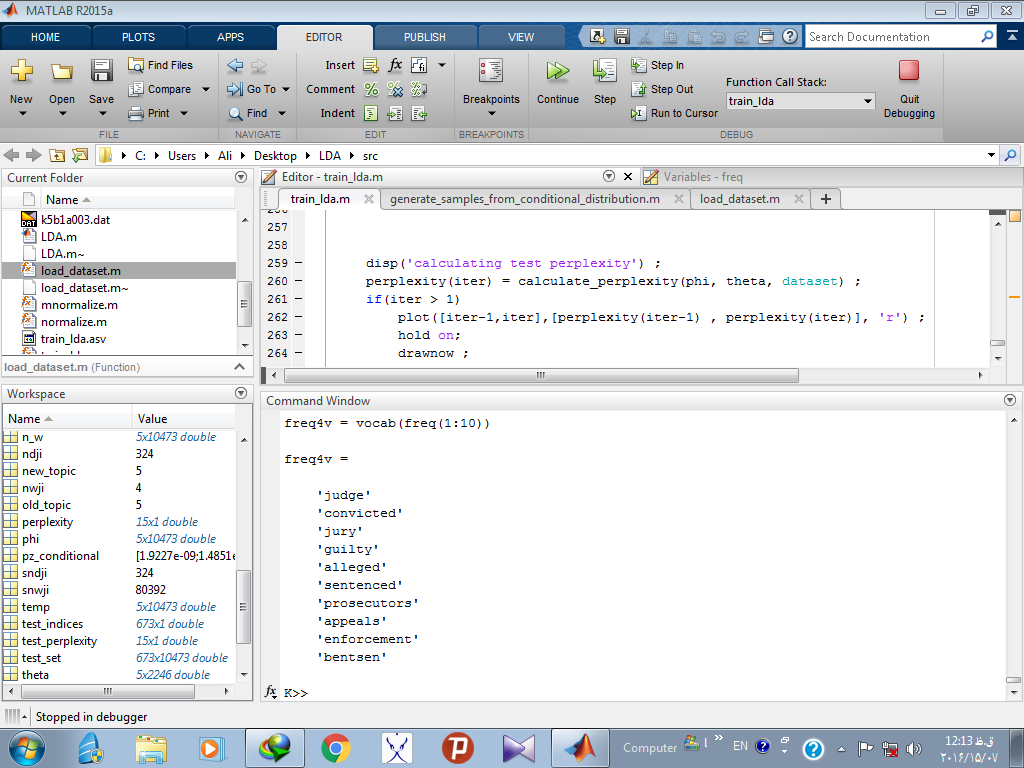
\includegraphics[scale=0.25]{Imgs/freqk4.png}
		\caption{کلمات شاخص عنوان چهارم}
	\end{subfigure}
	\begin{subfigure}{.45\textwidth}
%		\center
		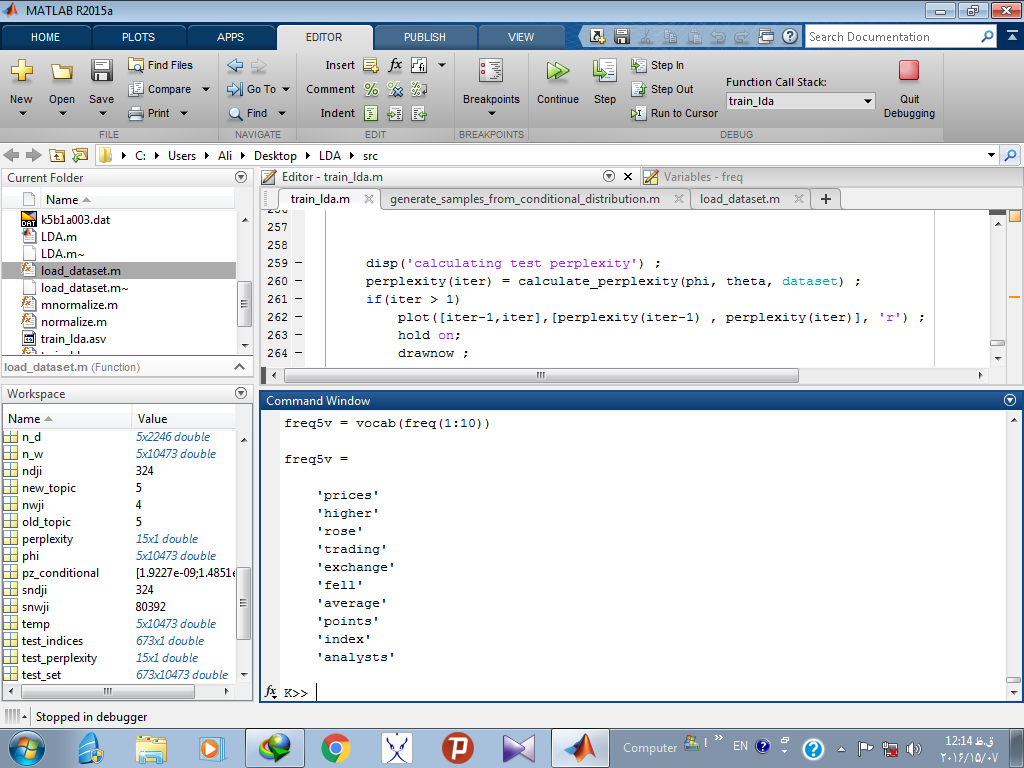
\includegraphics[scale=0.25]{Imgs/freqk5.png}
		\caption{کلمات شاخص عنوان پنجم}
	\end{subfigure}
\caption{کلمات شاخص ۵ عنوان
}
\label{fig:wordcluster}
\end{figure} 



%%%%%%%%%%%%%%%%%%%%%%%%%%%%%%%%%%%%%%%%%%%%%%%%%%%%%%%%%%%%%%%%%%%%%%%%%%%%%%%%%%%
\vfill
\section{توضیحات}
\begin{itemize}
\item [*] با توجه به ز مان‌بر بودن اجرای کامل الگوریتم، عموم آزمایشات نتیجه ۶۰ تکرار اول الگوریتم  را گزارش داده‌اند. بدیهی  است ادامه اجرای الگوریتم بر بهبود پاسخ موثر خواهد بود اما نتایج مقایسات تغییری نخواهند کرد. 
\item [*] سورس کد مربوط به پروژه در ضمیمه این گزارش ارسال شده است. همین‌طور این کد از
\href{https://github.com/ahmad-asadi/PGM/tree/master/LDA}
{این لینک}
، قابل 
دریافت می‌باشد.
%\item [*] آدرس لینک برای دریافت کد:
%\LTR{
%\url{https://github.com/ahmad-asadi/PGM/tree/master/BayesianNetwork}
%}
\end{itemize}




\end{document} 
